\documentclass[11pt]{article}

\usepackage{amsmath}
\usepackage{textcomp}
\usepackage[top=0.8in, bottom=0.8in, left=0.8in, right=0.8in]{geometry}
% add other packages here
\usepackage{amssymb}
\usepackage{bbm}
\usepackage{caption}
\usepackage{amsmath}
\usepackage{graphicx}

\DeclareMathOperator*{\argmax}{arg\,max}

% put your group number and names in the author field
\title{\bf Exercise 2: A Reactive Agent for the Pickup and Delivery Problem}
\author{Group \textnumero 54: Oriol Barbany Mayor, Natalie Bolón Brun}

% the report should not be longer than 3 pages

\begin{document}
\maketitle

\section{Problem Representation}

\subsection{Representation Description}
The topology of the problem is defined by the weighted graph $\mathcal{G}=(V,E)$, where $V$ is the set of cities and $E$ represent the roads between them, which have a weight function $w:E\to \mathbb{R}^+$ associated representing the distance in kilometers between vertices connected by an edge. To ease the notation, we define $d(s,s')$ to be the distance between city $s$ and city $s'$. Note that if $(s,s')\in E$, $d(s,s')=w(s,s')$ and otherwise it is the minimum length path between them. Given the pickup and delivery problem presented, we have defined the states and actions as follows.
 
\textbf{States}: Our state space is the set of cities in the problem, i.e. $\mathcal{S} = V$. The state of the agent at a given time step corresponds to the city where it is currently located.

\textbf{Actions}: The actions are represented by a tuple of two elements: Accept/Refuse and the destination city. Note that a given task can have any destination except the source, and if the task is refused, we restrict the next movement to neighbor cities. We apply this constraint in order to avoid changing the action chosen by the policy if a new task is found when going from the source to the destination without a task.

Formally, our action set for a city $s\in V$ is $\mathcal{A}(s) = \{Accept\} \times V \setminus s \cup \{Refuse\} \times \mathcal{N}(s)$, where $\mathcal{N}(s)$ is the set of neighbors of city $s$. We consider all the set of actions when computing the Q-values, but in the simulation, not all the actions are available in all cities. Indeed, there is at most one $\{Accept\}$ action, so the set of possible actions $\mathcal{A}(s)$ will be constrained. On the one hand, if there is no task available in $s$ for a given time step, the possible actions will be limited to the subset $\{Refuse\} \times \mathcal{N}(s)$. We then define $Best(s)$ to be the best action of this restricted set. 

On the other hand, if there is a task to city $s'\in V\setminus s$, then $\mathcal{A}(s)$ will be constrained to $\{Accept\} \times \{s'\} \cup \{Refuse\} \times \mathcal{N}(s)$. Hence, in this case best action will be $\arg\max \{Best(s), \{Accept\} \times \{s'\}\}$. 

\textbf{Reward table}: The rewards are given by two factors: the actual reward of pursuing a task from $i$ to $j$ given by $r[i,j]$, a table accessed through the \texttt{TaskDistribution} object, and the cost of movement. Let $c$ be the cost per kilometer, then we compute the reward for each state-action pair as follows:

\begin{align}
    R(s, a) = r[s, \pi_2(a)] \mathbbm{1}\{\pi_1(a) = Accept\}- c \cdot d((s, \pi_2(a)))
\end{align}
, where $\mathbbm{1}\{\cdot\}$ is the indicator function and $\pi_i$ is the projection operator defined by $\pi_1(x, y) = x$, $\pi_2(x, y) = y$. In the case of an action $a$ from an state $s$, $\pi_1\in \{Accept, Reject\}$ and $\pi_2(a) \in V \setminus s$ (the destination city). Note that $d((s, \pi_2(a)))$ is the distance from city $s$ to the destination city, i.e. the kilometers separating them.

%% NO ESTEM TENINT EN COMPTE EL PES DEL PAQEUT PERQ SI FOS MENYS DE 1 SURTIRIA MÉS BARAT PORTAR PAQUET Q NO POTAR-NE! 
%% SHOULD WE CHECK CAPACITY? 

\textbf{Probability transition table:} This table represents the probability to reach a city $s'$ through action $a$ starting at city $s$. In our case, $p[i,j]$, a table accessed through the \texttt{TaskDistribution} object, gives the probability of having a task from city $i$ to city $j$.

\begin{align}
    T(s,a,s')=
    \begin{cases}
        p[s,s'] & \text{if } \pi_1(a)=Accept \\
        \frac{1}{|\mathcal{N}(s)|}(1 - \sum_{s'\in V\setminus s} p[s,s']) &\text{otherwise}\\
    \end{cases}
\end{align}

Note that $\pi_1(a)=Refuse$ only for actions leading to neighbor states, so by our formulation, we make sure that
\begin{displaymath}
    \sum_{a \in\mathcal{A}(s)} T(s,a,s'=\pi_2(a))=1 \quad  \forall s
\end{displaymath}
and when we don't have task, the probability to move to any neighbor city is uniform.
% describe how you design the state representation, the possible actions, the reward table and the probability transition table

\subsection{Implementation Details}
% describe the implementation details of the representations above and the implementation details of the reinforcement learning algorithm you implemented
The stopping criteria for the iterative computation of the Q-values and V-values is based on the absolute value of the difference between the previous and the updated Q-value, which we will denote $\Delta_q(t)$ for iteration $t$. We don't consider the difference of V-values since
\begin{align*}
    |V_{t+1}(s) - V_{t}(s)| &= |\max_a Q_{t+1}(s,a) - \max_a Q_{t}(s,a) | \leq \max_a \{|Q_{t+1}(s,a) - Q_{t}(s,a)|\} \\
    &\leq \max_{s,a} \{|Q_{t+1}(s,a) - Q_{t}(s,a)|\} := \Delta_q(t+1)
\end{align*}
so the difference in Q-values will also be bigger than those of V-values. Hence, we take the maximum absolute difference between Q-values when updating all the values for all state-action pair, and if it's bigger than $\varepsilon=10^{-5}$ we perform another iteration of all the values until the stopping criteria is satisfied, i.e. until iteration $t$ such that $\Delta_q(t) \leq \varepsilon$.

\section{Results}
% in this section, you describe several results from the experiments with your reactive agent

\subsection{Experiment 1: Discount factor}
% the purpose of this experiment is to understand how the discount factor influences the result
Different discount factors have been used to understand its influence in the system. 

\subsubsection{Setting}
The experiment has been conducted with 7 different agents. Each of them was assigned a different discount factor ranging from 0 to 0.95. Moreover, in order to enhance the influence of the discount factor in the cumulative reward, two different experiments were conducted: one with the initial cost of 5u/km and a second one with a cost of 50u/km. 
% you describe how you perform the experiment (you also need to specify the configuration used for the experiment)

\subsubsection{Observations}
% you describe the experimental results and the conclusions you inferred from these results


\begin{minipage}[]{\textwidth}

\begin{minipage}[]{0.48\textwidth}
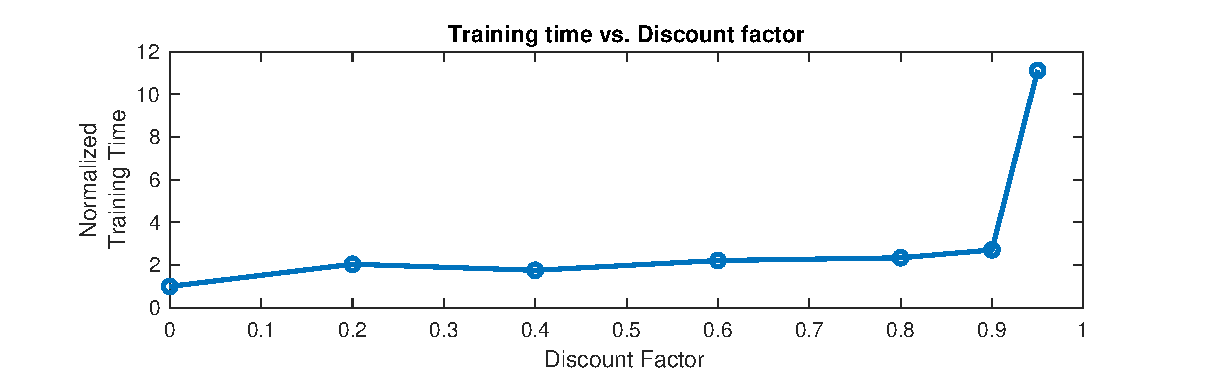
\includegraphics[width=\textwidth]{2-reactive/doc/plots/time-discount-2.eps}
\captionof{figure}{Evolution of training time for different discount factors}
\label{fig:time}
\end{minipage}
\hfill
\begin{minipage}[]{0.5\textwidth}
The first effect we can see is the influence in the training time. As we can see in Figure \ref{fig:time}, the time required to converge when computing the Q values increases as we increase the discount factor. If we select as reference the time required for a discount factor of 0, we can see that for higher discounts up to 0.9, this time doubles. Once we overpass this late value, the required time for training increases much faster, resulting in 7 times more time than the base case for a discount of 0.95. \\
\end{minipage}

\end{minipage}

%% afegir plots discount vs time i discount vs revenue


On the other hand, the discount value also has an impact in the average total revenue. This factor reflects how much importance we give the future possible rewards vs. the current one. Therefore, it determines which actions will our agent perform. We have studied 2 different cases, varying the cost per km of the vehicles to point out the influence of the discount factor. 

For low values of cost, we can see that the difference between the policies performance is not very relevant and all agents achieve a similar reward. It is not the same case when we increase the cost per km. In this case, the gap in revenue achieved between large or small discount factors increases, pointing out the need of a non-zero value to improve performance. 


\begin{minipage}[]{\textwidth}

\begin{minipage}[]{0.45\textwidth}
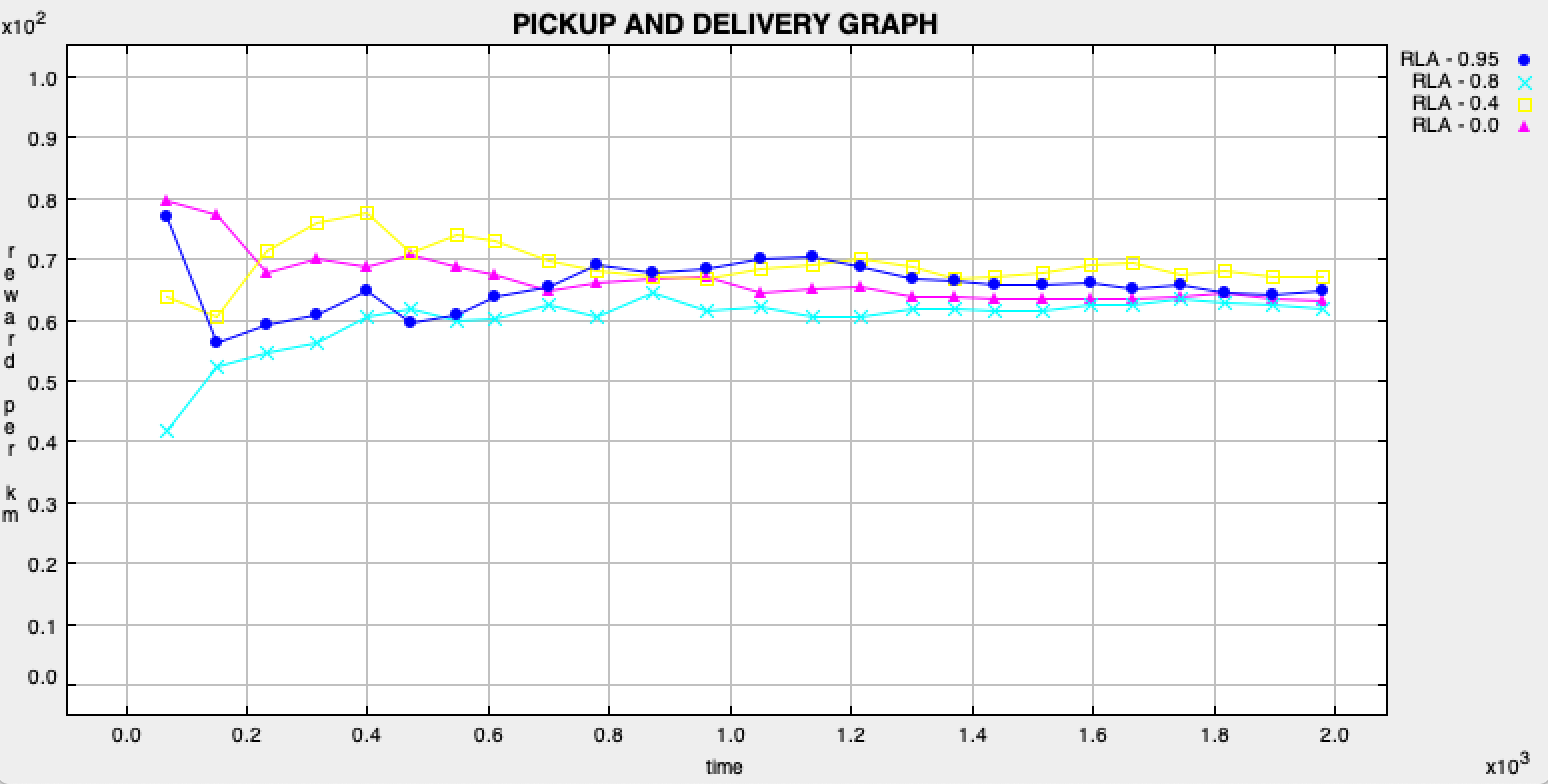
\includegraphics[width=\textwidth]{2-reactive/doc/plots/2000ticks-cost5.png}
\captionof{figure}{Evolution of reward per km with  \\cost = 5u/km}
\label{fig:cost5}
\end{minipage}
\hfill
\begin{minipage}[]{0.45\textwidth}
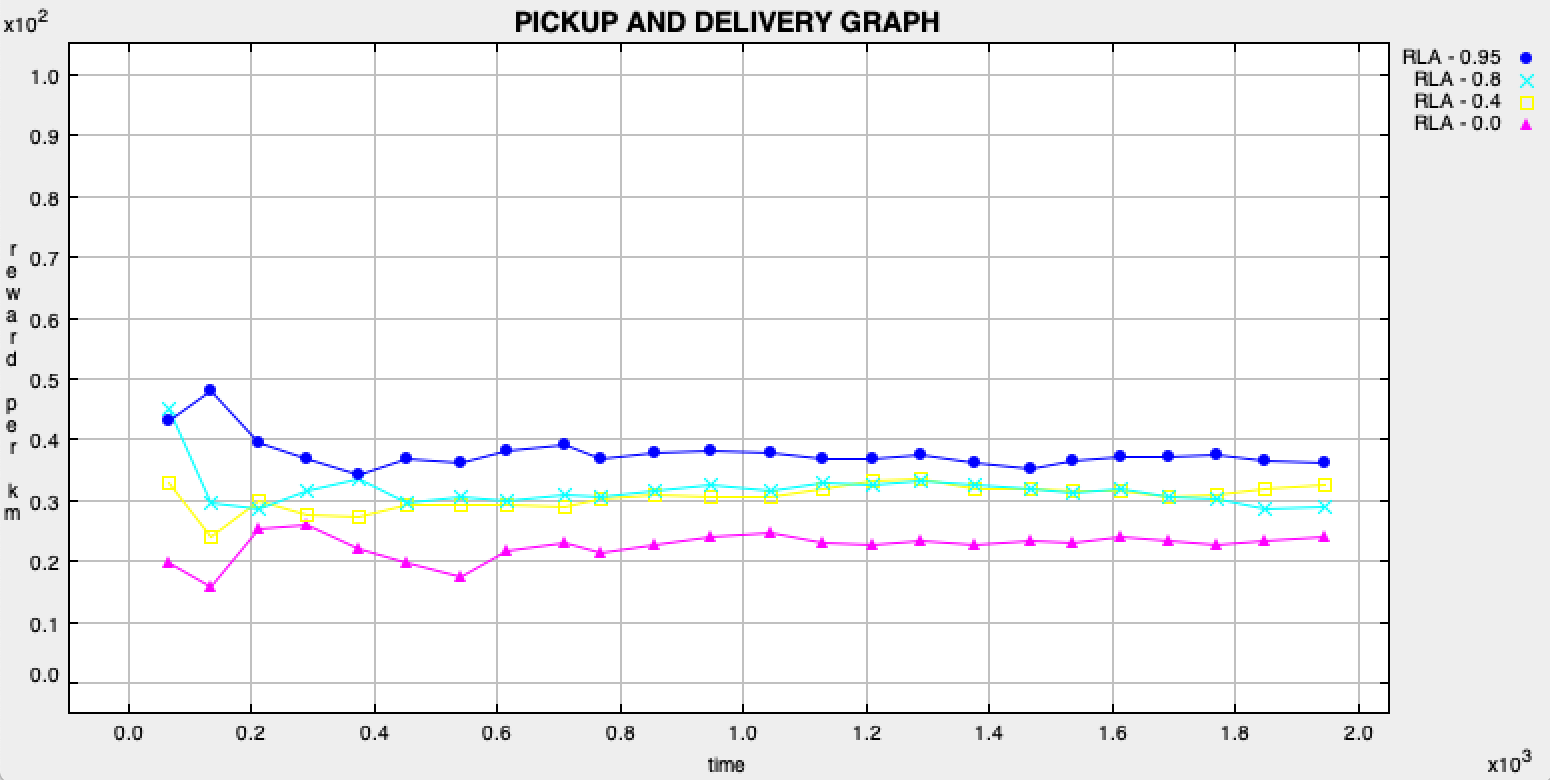
\includegraphics[width=\textwidth]{2-reactive/doc/plots/2000ticks-cost50.png}
\captionof{figure}{Evolution of reward per km with  \\cost = 50u/km}
\label{fig:cost50}
\end{minipage}
\hfill

\end{minipage}



\subsection{Experiment 2: Comparisons with dummy agents}
% you compare the results of your agent with two dummy agents: the random agent that was already given in the starter files and another dummy agent that you define and create. You should report the results from the simulations using the topologies given in the starter files and optionally, additional topologies that you create.

\subsubsection{Setting}
% you describe how you perform the experiment and you describe the dummy agent you created (you also need to specify the configuration used for the experiment)
To evaluate the performance of the reactive agent, it is compared with two other agents: the random agent already provided and the dummy agent. The dummy agent is such that it only moves to neighboring cities. When located in a city, the agent will accept a task only if its destination is a neighbor city. Otherwise, if there is no task or the destination is not among its neighbors, it move to a city selected randomly among its neighbors with equal probability. 

The capacity of the vehicles is left much higher than the weight of the packets. The cost per km is left to 5u/km. For the dummy agent, the pickup probability is set to 0.85 while the discount factor for the reactive agent is set at 0.8. 

\subsubsection{Observations}
% elaborate on the observed results
\begin{minipage}[]{\textwidth}

\begin{minipage}[]{0.48\textwidth}
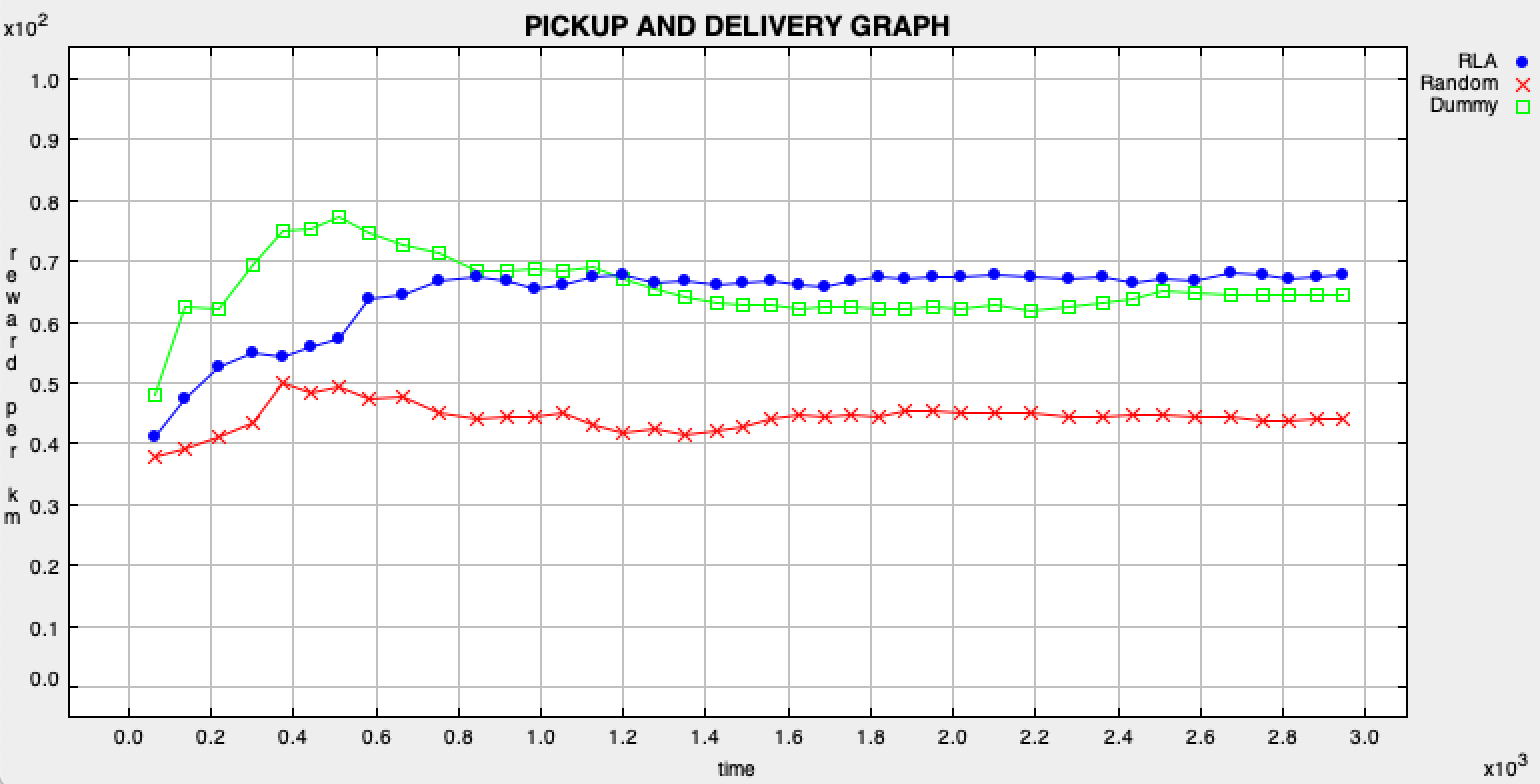
\includegraphics[width=\textwidth]{2-reactive/doc/plots/rla-dummy.png}
\captionof{figure}{Evolution of reward per km for three different agents}
\label{fig:rla}
\end{minipage}
\hfill
\begin{minipage}[]{0.5\textwidth}
Given the results on Figure \ref{fig:rla}, we can see that the worst performing agent is the random one. The other two agents are following a policy with the aim to obtain the maximum average accumulated reward. In this case, the reactive agent achieves a higher reward although the dummy agent is quite close in terms of performance. This can be explained since the dummy agent will reduce its travel cost by not accepting tasks implying long distance travels and still, given the size and connectivity of the graph, it has high probability to find tasks between neighbor cities. In this case, the strategy designed imposing an intuitive behaviour produces a similar behaviour to the one obtained by optimizing an average reward. 
\end{minipage}

\end{minipage}


\end{document}
